% \documentclass{book}

\documentclass[12pt]{article}
\usepackage[pdfborder={0 0 0.5 [3 2]}]{hyperref}%
\usepackage[left=1in,right=1in,top=1in,bottom=1in]{geometry}%
\usepackage[shortalphabetic]{amsrefs}%
\usepackage{amsmath}
\usepackage{enumerate}
\usepackage{enumitem}
\usepackage{amssymb}                
\usepackage{amsmath}                
\usepackage{amsfonts}
\usepackage{amsthm}
\usepackage{bbm}
\usepackage[table,xcdraw]{xcolor}
\usepackage{tikz}
\usepackage{float}
\usepackage{booktabs}
\usepackage{svg}
\usepackage{mathtools}
\usepackage{cool}
\usepackage{url}
\usepackage{graphicx,epsfig}
\usepackage{makecell}
\usepackage{array}

\def\noi{\noindent}
\def\T{{\mathbb T}}
\def\R{{\mathbb R}}
\def\N{{\mathbb N}}
\def\C{{\mathbb C}}
\def\Z{{\mathbb Z}}
\def\P{{\mathbb P}}
\def\E{{\mathbb E}}
\def\Q{\mathbb{Q}}
\def\ind{{\mathbb I}}

\graphicspath{ {images10/} }

\begin{document}

\section*{16 March 2017}

\subsection*{Symmetry Issues}
Before exploring symmetry of eigenfunctions, I though I would take a look at the symmetry of the single and double pulse solutions, just to make sure. We know that the stationary single and multi-pulse solutions should be symmetric about a vertical axis (usually $x = 0$, unless the wave has translated), so we attempt to verify that this is the case. We also know that if $u(x)$ is a solution to the system, then so is $u(-x)$, i.e. the system obeys reflection symmetry. This can easily be shown.\\

We first take a look at the initial single pulse $u(x)$ where the exact solution is known ($c = 0.2130$). We use finite difference methods, Neumann BCs, domain size $L = 50$, and grid size $N = 2000$. (The numerical method doesn't really matter here, since what we will show happens for all numerical methods.) If we plug $u(-x)$ into the 5th order ODE, the max of the result is the same as if we plug in $u(x)$ (it should be 0), so $u(-x)$ is also a solution. Now, let's test for symmetry. Subtracting $u(-x)$ from $u(x)$, we get the following plot.

\begin{figure}[H]
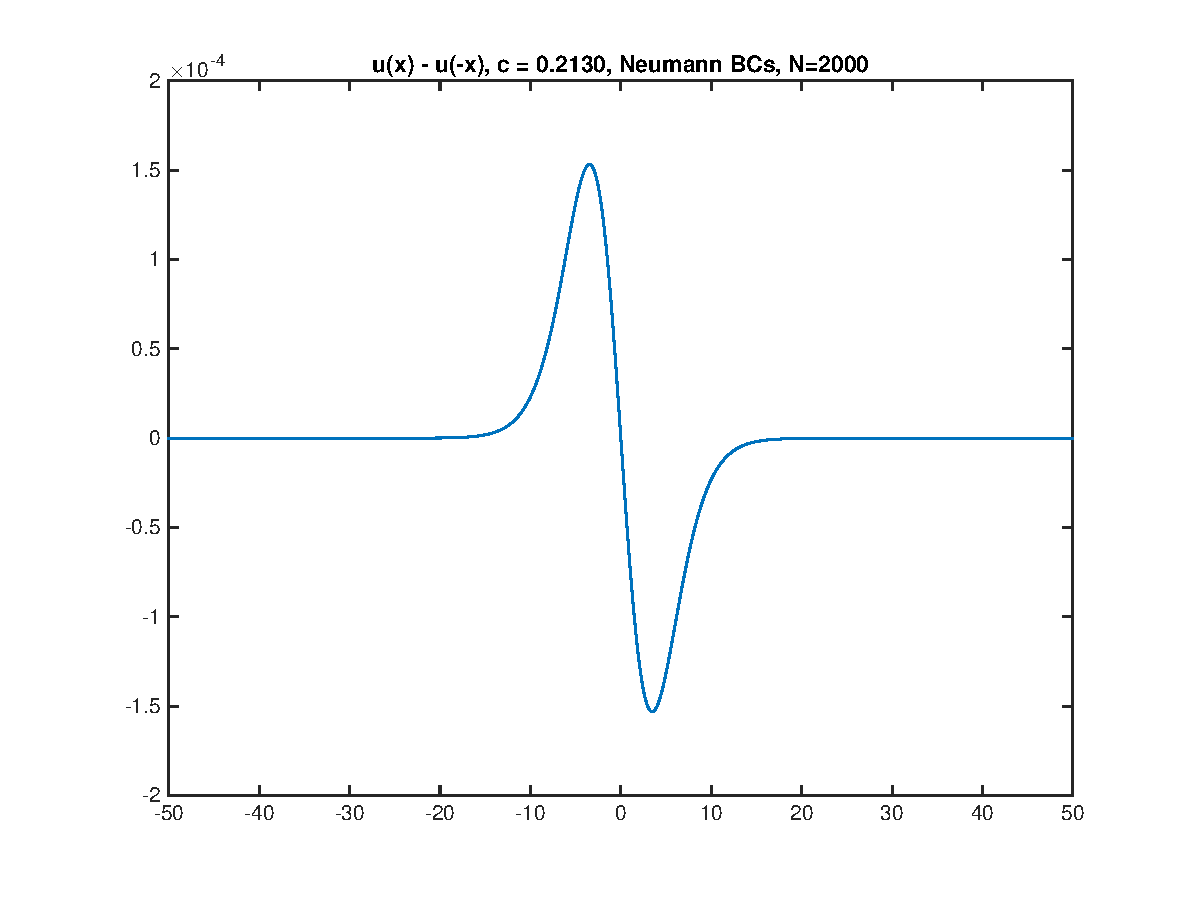
\includegraphics[width=8.5cm]{0singleflipdiffneumann}
\end{figure}

This looks a lot like a rescaled version of the derivative of the single pulse. To confirm this, we will plot a normalized version of this and a normalized version of the derivative on a single plot; they are indistinguishable.

\begin{figure}[H]
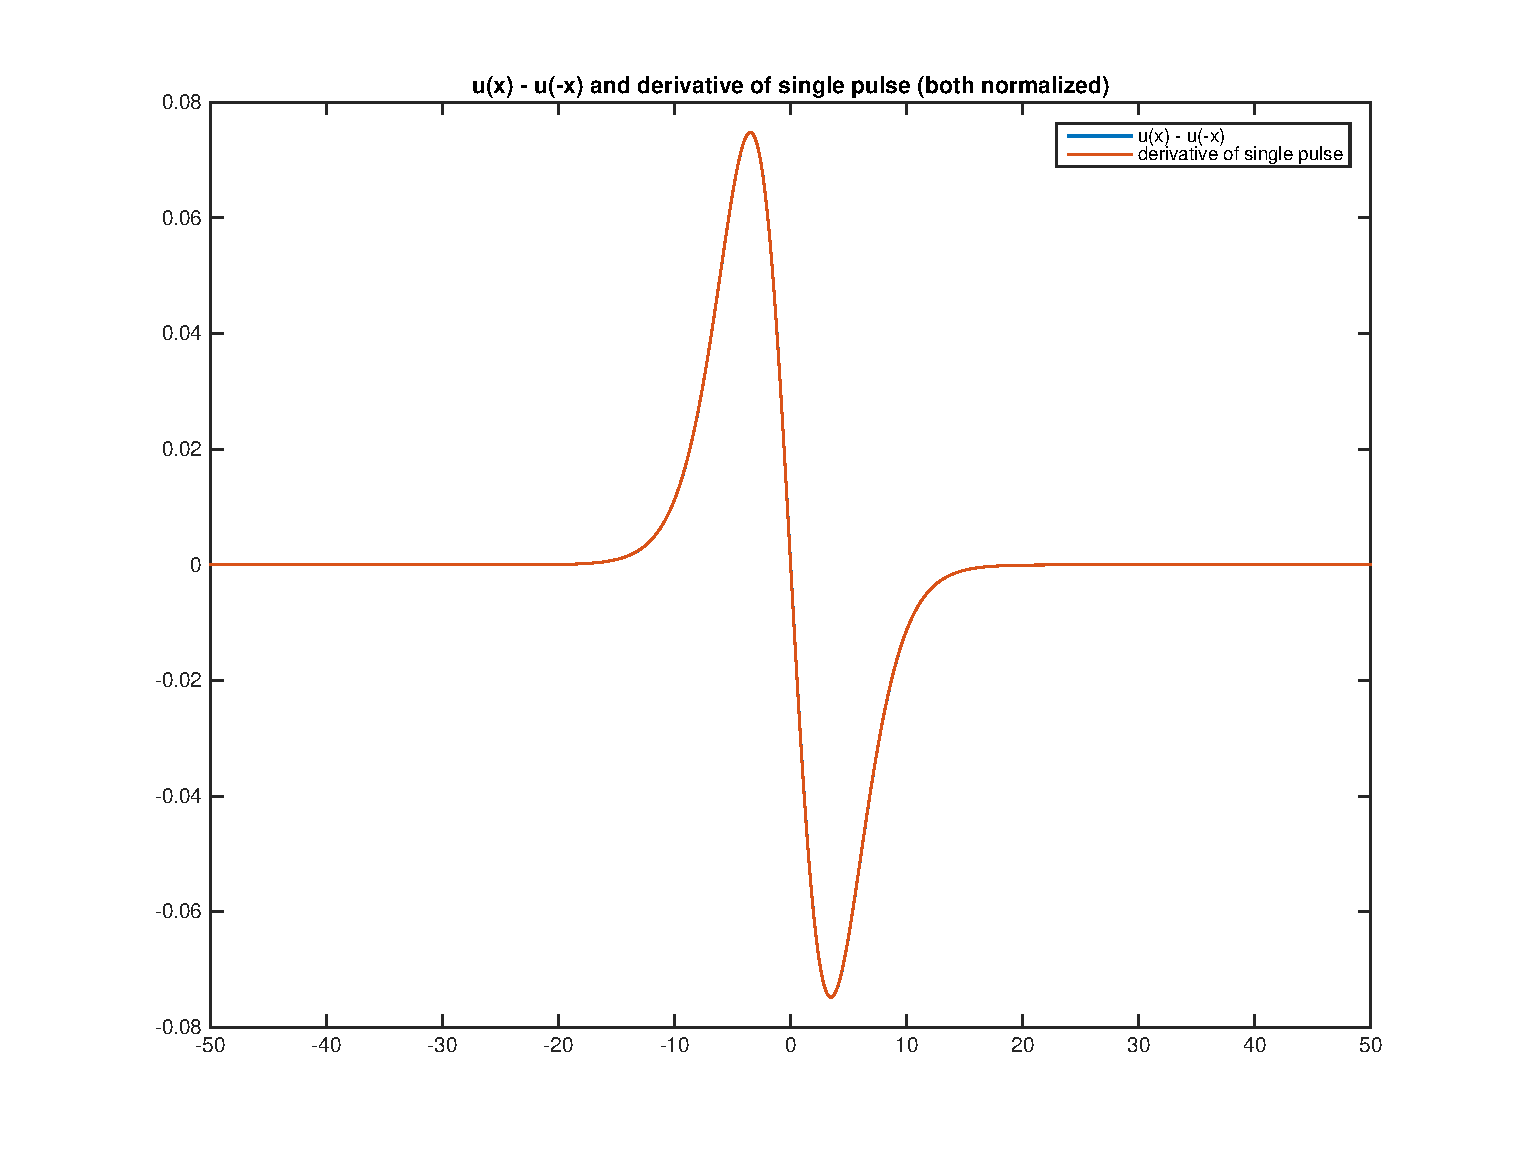
\includegraphics[width=8.5cm]{0singleflipdiffandderivneumann}
\end{figure}

This same phenomenon occurs for all pulses (single and double), all numerical methods, and all boundary conditions. Weirdly, if we use more grid points, the magnitude of this assymetry grows, i.e. if we take $u(x) - u(-x)$, with more grid points we get a larger scaled version of the derivative. This is also true in all situations. \\

Since this is not supposed to happen, the questions are: (1) Can we get rid of this, i.e. make the solutions symmetric, and (2) Does it matter? For the first question, note that the derivative of the pulse is an odd function, so $u(x) + u(-x) = 0$. Since essentially all the assymetry is an odd function, then we should be able to take the average of $u(x)$ and $u(-x)$ to get rid of it, i.e. replace $u(x)$ by $\frac{1}{2}(u(x) + u(-x))$. This does in fact work. If we do that and run it through \texttt{fsolve}, here's what we get (initial single pulse, comparison between Neumann and Fourier).

\begin{figure}[H]
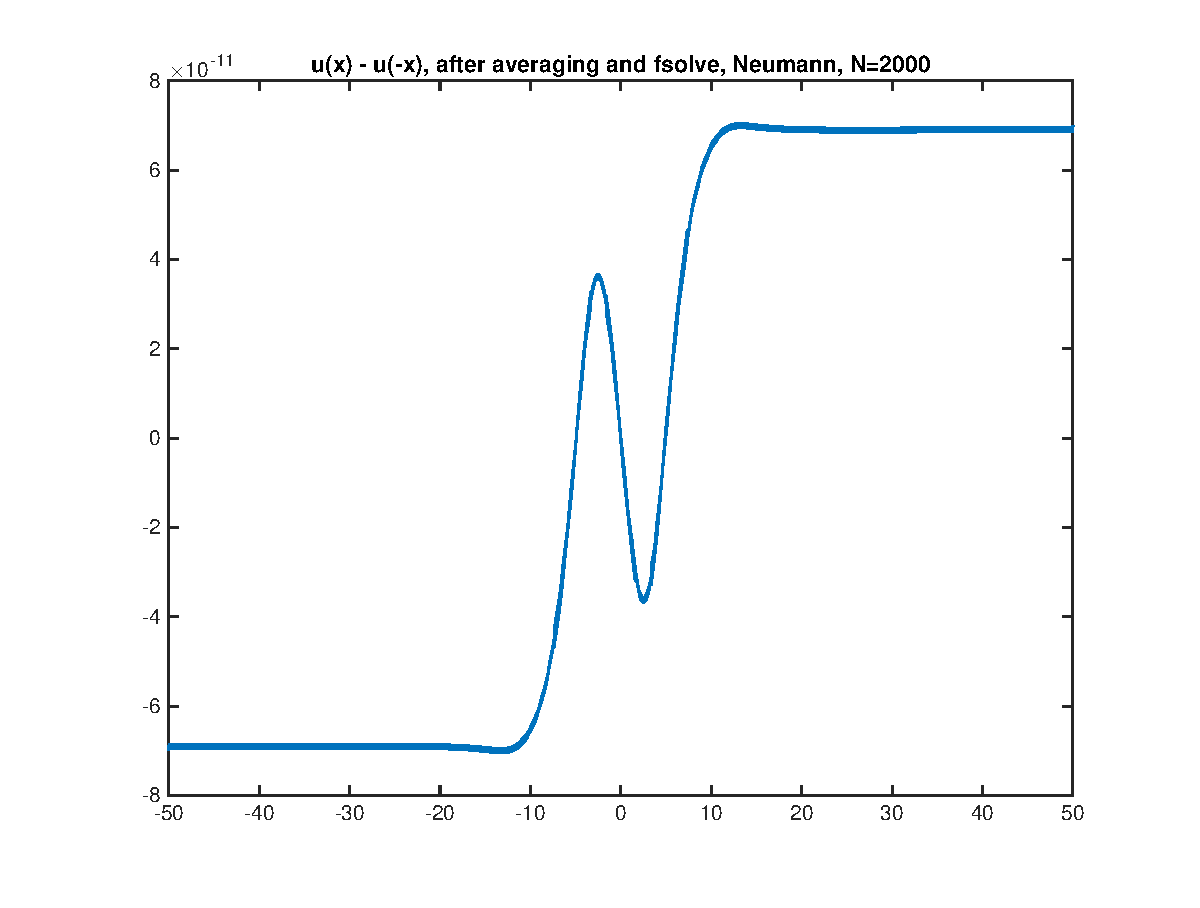
\includegraphics[width=8.5cm]{0singleflipdiffneumannavgfsolve}
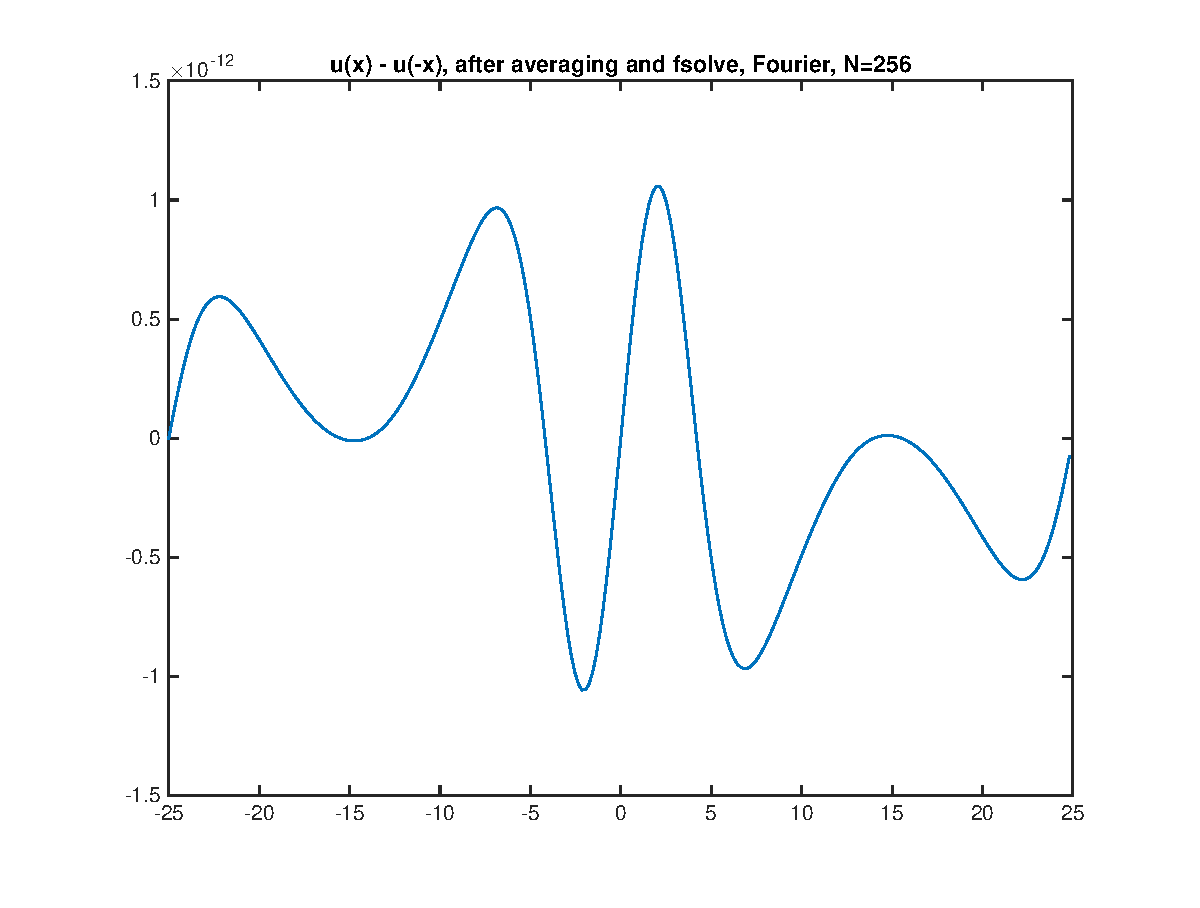
\includegraphics[width=8.5cm]{0singleflipdifffourieravgfsolve}
\end{figure}

Fourier looks a little better (so it's good that is what we are using), but both are within the realm of machine precision. \\

Before we continue, here is an interesting observation. Take the symmetric wave we obtained above from averaging; call it $v(x)$. By construction, this wave is perfectly symmetric about the $y$-axis, so $v(x) - v(-x) = 0$. Now let's look at $v(x+\epsilon) - v(-x)$, where $\epsilon$ is the mesh size. A plot of this also looks like the derivative. Here is a plot of both functions normalized on the same plot.
\begin{figure}[H]
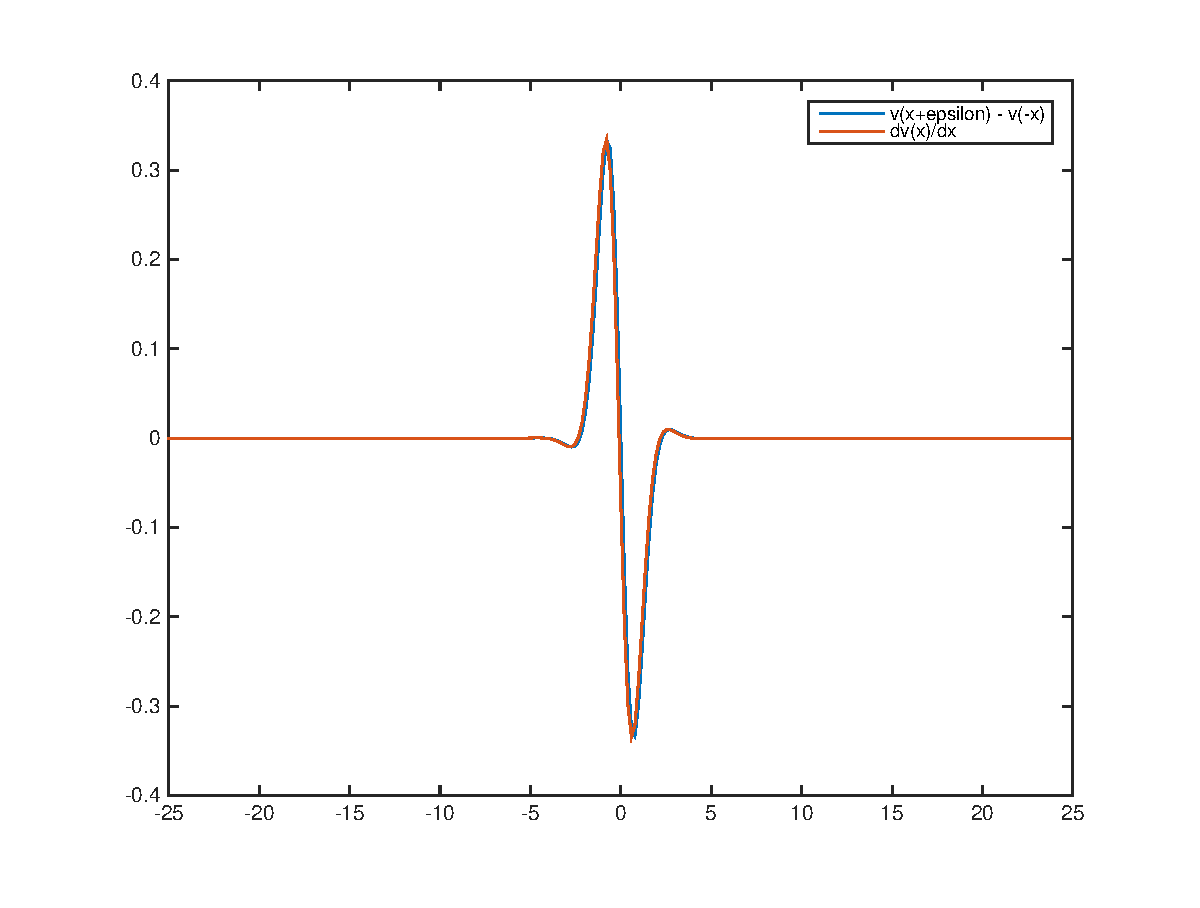
\includegraphics[width=8.5cm]{offsetflipdiff}
\end{figure}
They don't match exactly, but they are close. Maybe what is happening here is that \texttt{fsolve} is translating the solution by a very small amount, which affects symmetry about the $y$-axis but does not affect anything else since the equation is translation-invariant.\\

So we just need to see if any of this actually matters. Let's repeat one thing from before to see whether there is a difference. 

\subsection*{KdV, Double Pulse 2}
We use the KdV equation with $c = 40.9355$ and domain length $L = 25$. We use Fourier spectral methods starting at $N = 256$. We use an exponentially weighted space with weight $a = 0.2$ to separate the eigenvalues from the absolute spectrum. Here we show the Left Eignvalue (the one converging to the imaginary axis) together with the max of the absolute value of the eigenvalue problem $ (J -\lambda f)$ before and after using \texttt{fsolve} to get rid of the real part of the eigenvalue.

\begin{figure}[H]
\begin{tabular}{l|lll}
  $N$   &  Left Eigenvalue & $ \max (J -\lambda )f$ before \texttt{fsolve}  &  $\max (J -\lambda) f$ after \texttt{fsolve} \\ \hline
  256   &  1.7328e-06 + 0.6423i  &  3.4526e-11 &   1.6164e-08   \\ 
  512   &  1.7346e-06 + 0.6423i  &  2.0535e-09 &   1.1695e-08   \\ 
  1024  &  1.6914e-06 + 0.6423i  &  3.9923e-08 &   1.4544e-07   \\
  2048  &  3.4809e-06 + 0.6423i  &  2.0727e-06 &   1.2401e-06   \\
\end{tabular}
\end{figure}

This is not essentially any different than before. We can also use the unweighted space. Let's compare the eigenvalue we get linearizing about the nonaveraged pulse to the one we get linearizing about the averaged pulse.

\begin{figure}[H]
\begin{tabular}{l|ll}
  $N$   &  eigenvalue (nonaveraged pulse) & eigenvalue (averaged pulse) \\ \hline
  256   &  1.6239e-11  + 0.6423i   &  5.6710e-13 + 0.6423i  \\ 
  512   &  -3.2265e-10 + 0.6423i   &  1.4286e-10 + 0.6423i  \\ 
  1024  &  8.7075e-09  + 0.6423i   &  5.0214e-09 + 0.6423i  \\
  2048  &  5.4825e-07  + 0.6423i   &  -1.2932e-08 + 0.6423i  \\
\end{tabular}
\end{figure}

The values which should be near 0 are smaller for the averaged version. In all cases, we can use \texttt{fsolve} to remove the small real part. Let's look at the integral of the eigenfunction keeping $L = 25$.
\begin{figure}[H]
\begin{tabular}{l|ll}
  $N$   &  Integral of Eigenfunction & Abs Value of Integral \\ \hline
        &   $1.0e-06 *$         & $1.0e-06 *$ \\
  256   &    -0.6971 + 0.0125i  & 0.6972 \\ 
  512   &     0.2464 + 0.0067i  & 0.2465 \\ 
  768   &     0.1341 + 0.0028i  & 0.1341 \\
  1024  &    -0.0871 + 0.0086i  & 0.0876 \\
\end{tabular}
\end{figure}

We can plot the log of the absolute value of the integral versus the log of the mesh size and get a nice straight line with slope approximately 1.5. This is what we got before, except the line looks a little nicer and the slope is closer to 1.5. I still have no idea how to interpret this slope, though.

\begin{figure}[H]
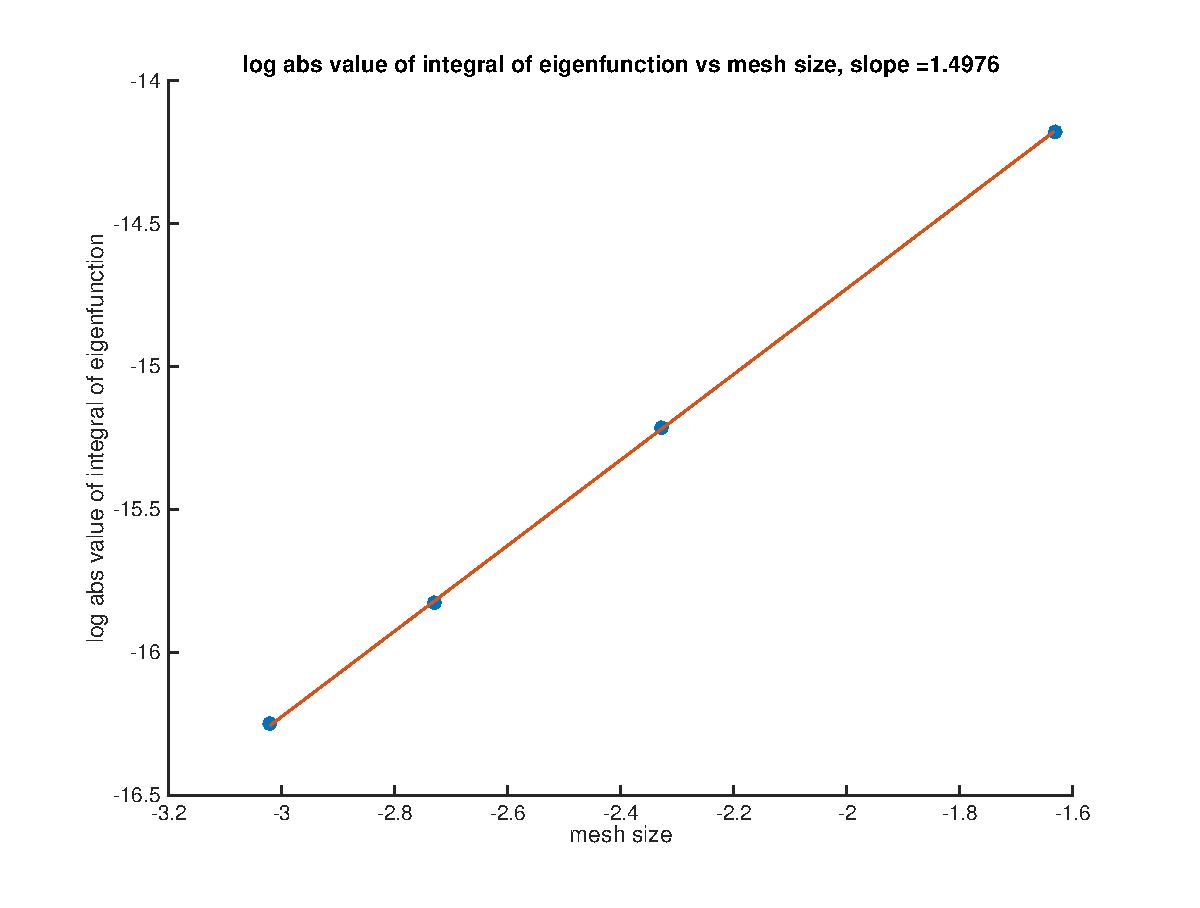
\includegraphics[width=8.5cm]{2doublelogabsintegralN}
\end{figure}

We still don't get anything nice if we keep the mesh size fixed at $N = 2048$ and vary the domain length $L$. Interestingly, for all but $L = 25$, the numbers are almost exactly the same as the case where we did not average.
\begin{figure}[H]
\begin{tabular}{l|lll}
  $N$   &  $L$ & Integral of Eigenfunction & Abs Value of Integral \\ \hline
        &   $1.0e-06 *$         & $1.0e-06 *$ \\
  2048  & 25    &  -0.0099 - 0.1898i &  0.1900 \\ 
  2048  & 50    &  -0.0449 + 0.0118i &  0.0464 \\ 
  2048  & 75    &   0.0622 + 0.0043i &  0.0624 \\
  2048  & 100   &   0.0875 + 0.0042i &  0.0876 \\
\end{tabular}
\end{figure}

Conclusion: this probably does not matter. 

\subsection*{Exponential Decay}
First, let's look at exponential decay of our various eigenfunctions. For this, we use the averaged solution, mostly because I don't see why not, although I'm not sure how much of a difference it really makes.

\subsubsection*{KdV, Double Pulse 1}
For comparison purposes, we first look at Double Pulse 1. First, here is a semilog plot (using log base 10, to make the graph easier to read) of the tail of Double Pulse 1.
\begin{figure}[H]
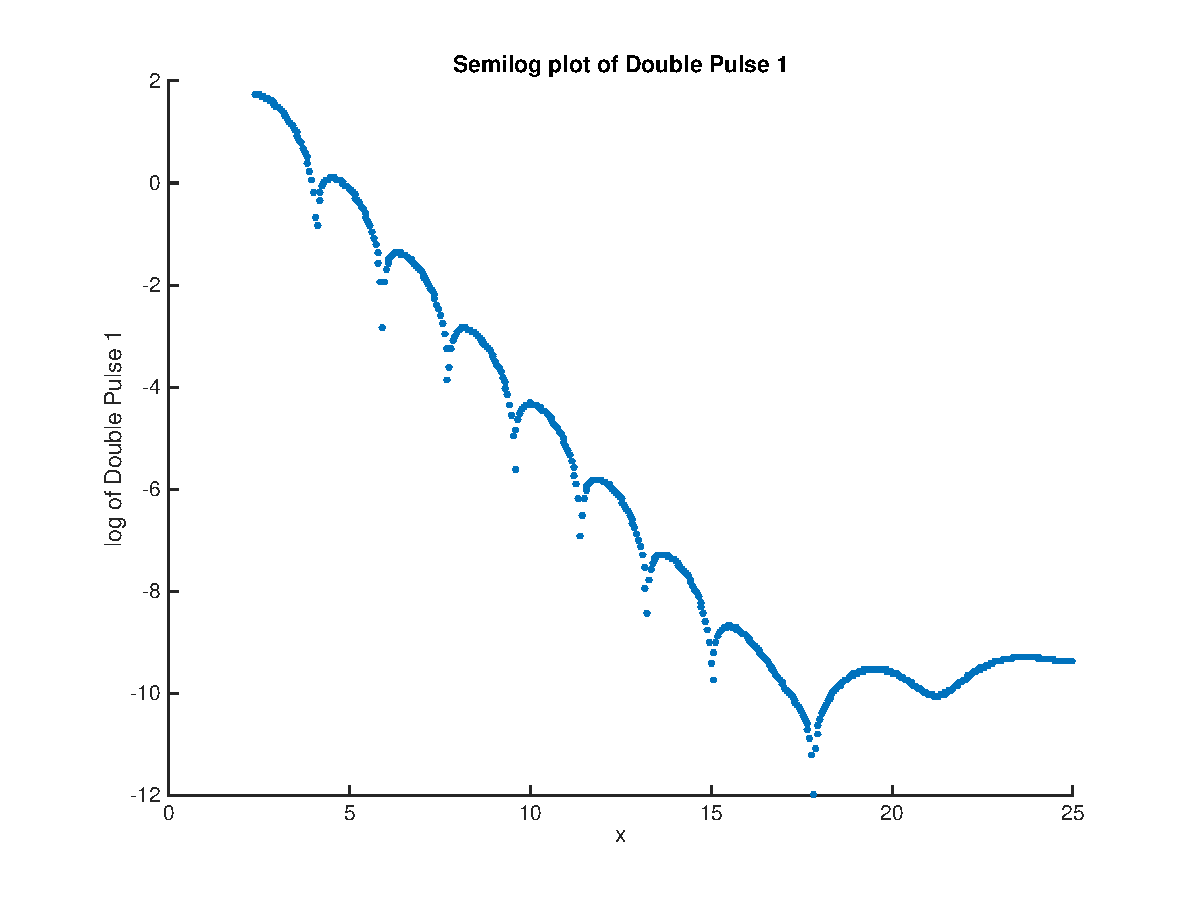
\includegraphics[width=8.5cm]{1doublesemilog}
\end{figure}
This shows a nice exponential decay trend. The tail levels off at order $1e-10$.\\

Compare this to a semilog plot of the eigenfunction corresponding to $\lambda = 3.4990$. For this, we use Fourier with $N = 1024$ and $L=25$. We initially have nice exponential decay, but it then stabilizes to a baseline that actually rises from order $1e-6$ to $1e-5$. If we repeat this for $L = 50$ (same $N=1024$), we have a similar plot, but it stabilizes to a baseline that rises from order $1e-7$ to $1e-6$.

\begin{figure}[H]
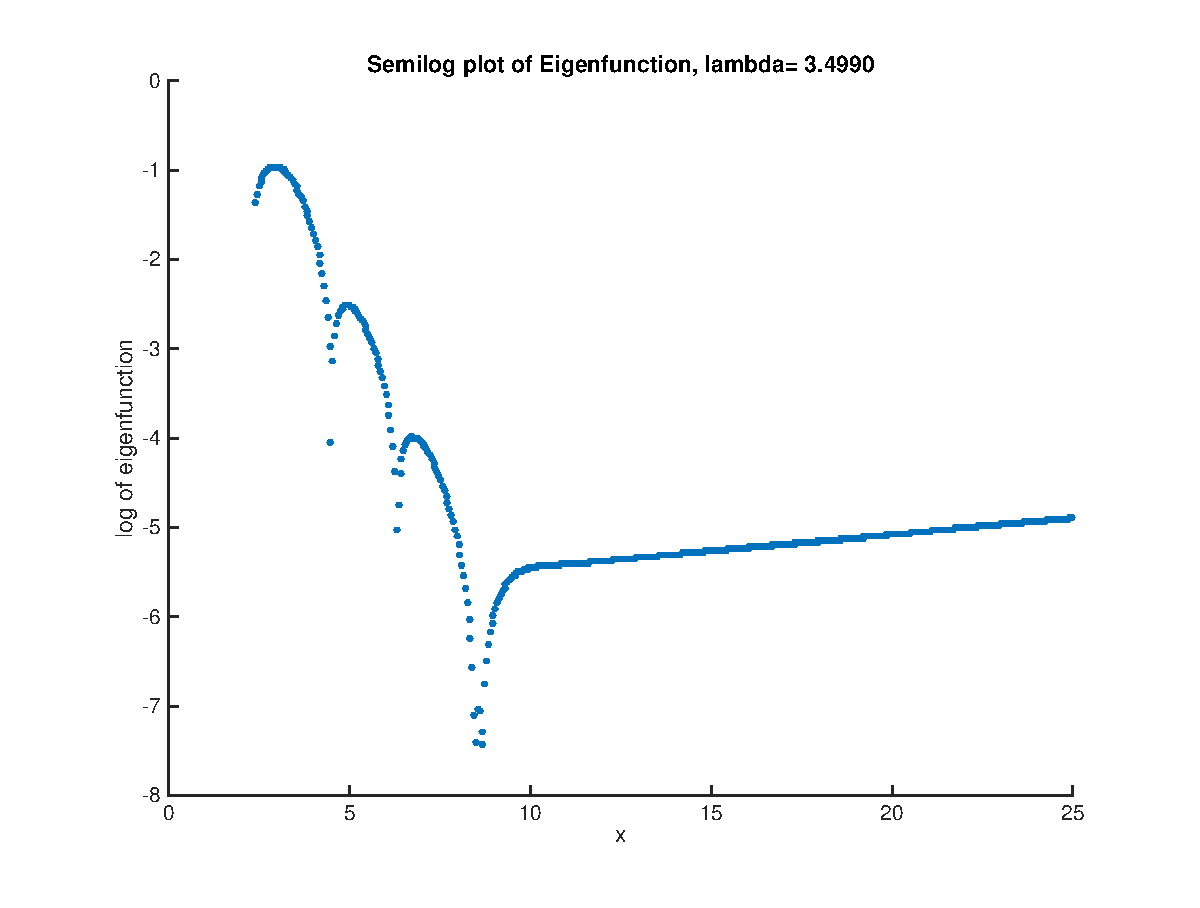
\includegraphics[width=8.5cm]{1doublesemilogeigenfn}
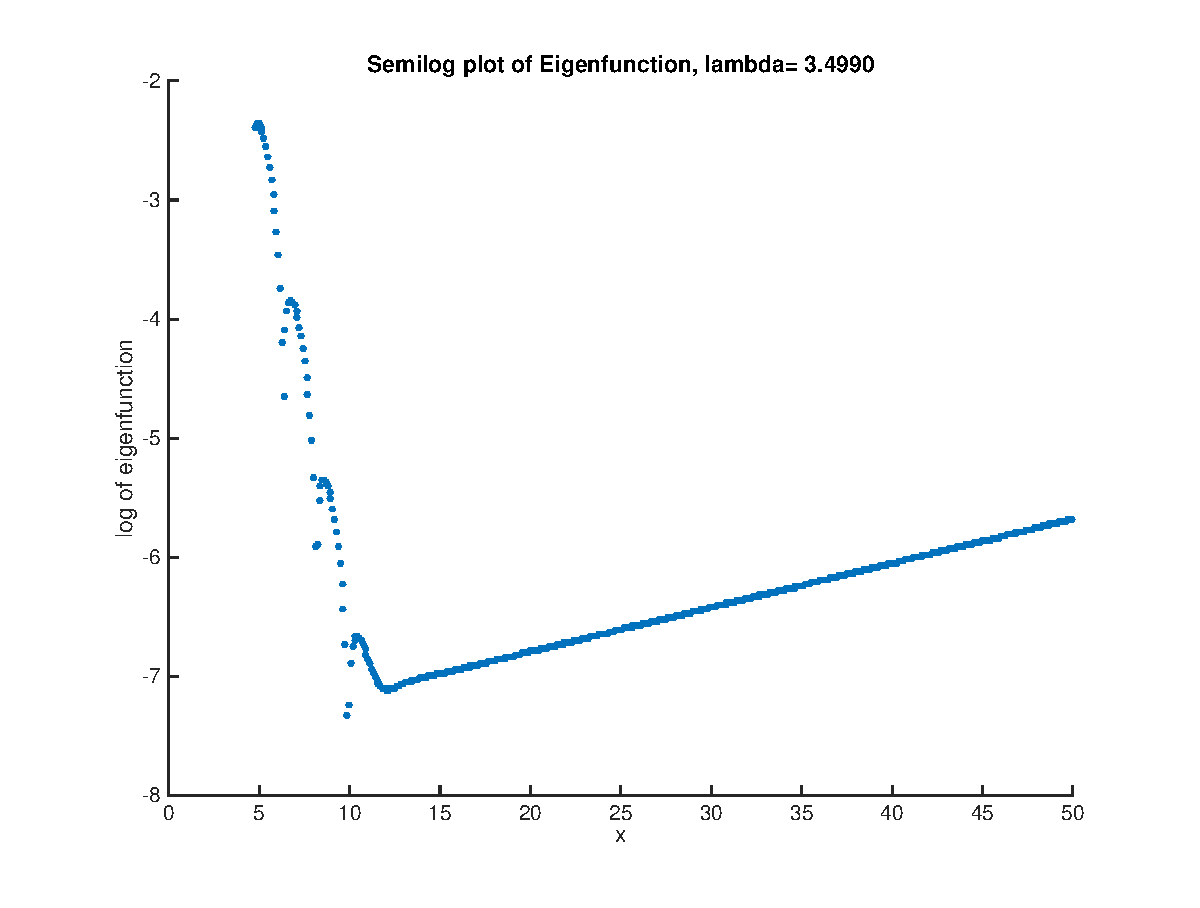
\includegraphics[width=8.5cm]{1doublesemilogeigenfn50}
\end{figure}

The same trend of upward-sloping baseline (but at a lower point) continues for $L = 1000$. Here we have to use $N=2048$ to get a reasonable eigenfunction. It does not matter whether or not we use the average wave.

\begin{figure}[H]
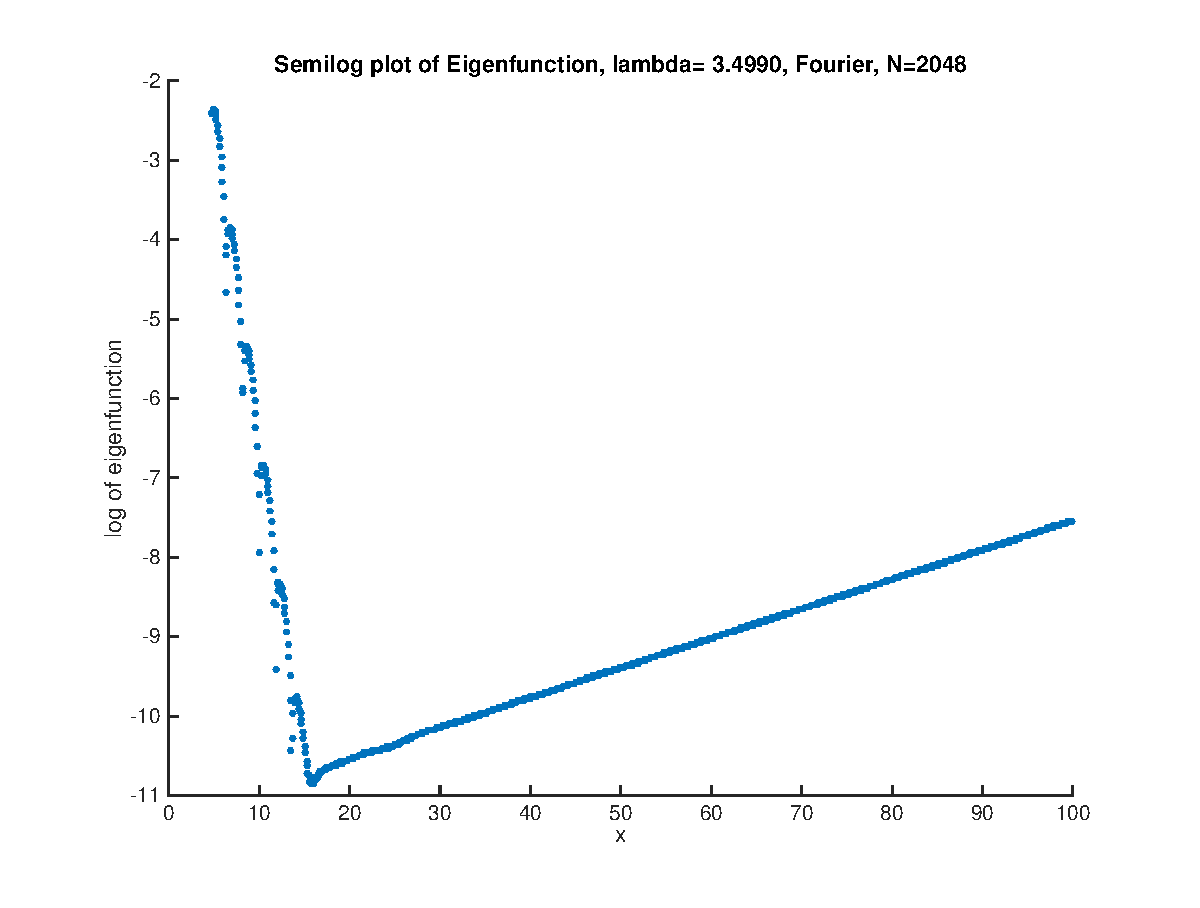
\includegraphics[width=8.5cm]{1doublesemilogeigenfn100_2048}
\end{figure}

So we have nice exponential decay, but I don't know what's up with the rising baseline. Luckily, this is not the double pulse we are most interested in.


\subsubsection*{KdV, Double Pulse 2}
We can do the same thing for Double Pulse 2. Here is a semilog plot of the tail of the double pulse, showing its exponential decay; decay pattern is very similar to Double Pulse 1.
\begin{figure}[H]
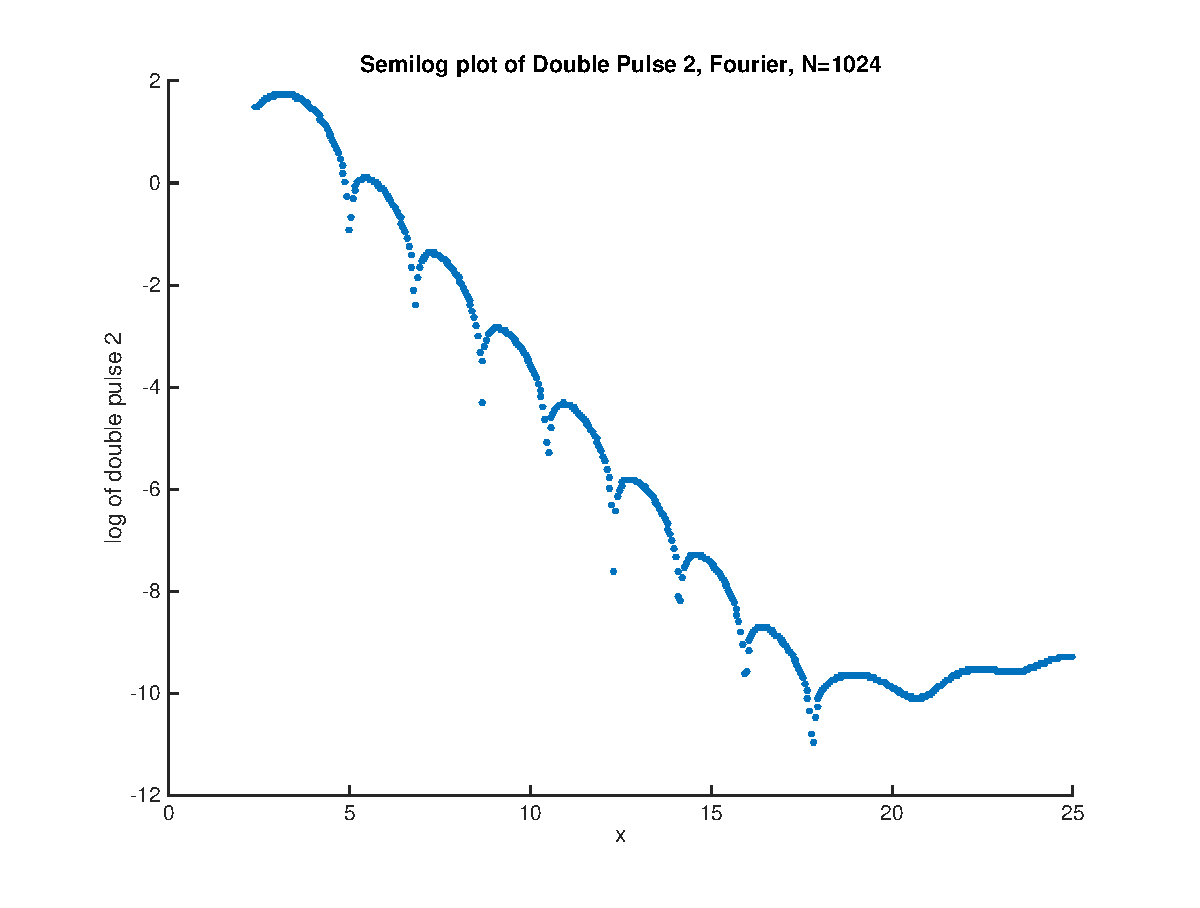
\includegraphics[width=8.5cm]{2doublesemilog}
\end{figure}

Here are semilog plots of the tail of the absolute value of the eigenfunction corresponding to $0.6423i$ for both $L = 25$ and $L = 50$. In both cases, we have exponential decay to a baseline, but in this case the baseline is flat. The baseline is at approximately $1e-6$ for both values of $L$. The baseline remains the same even if we increase $N$ (not shown).
\begin{figure}[H]
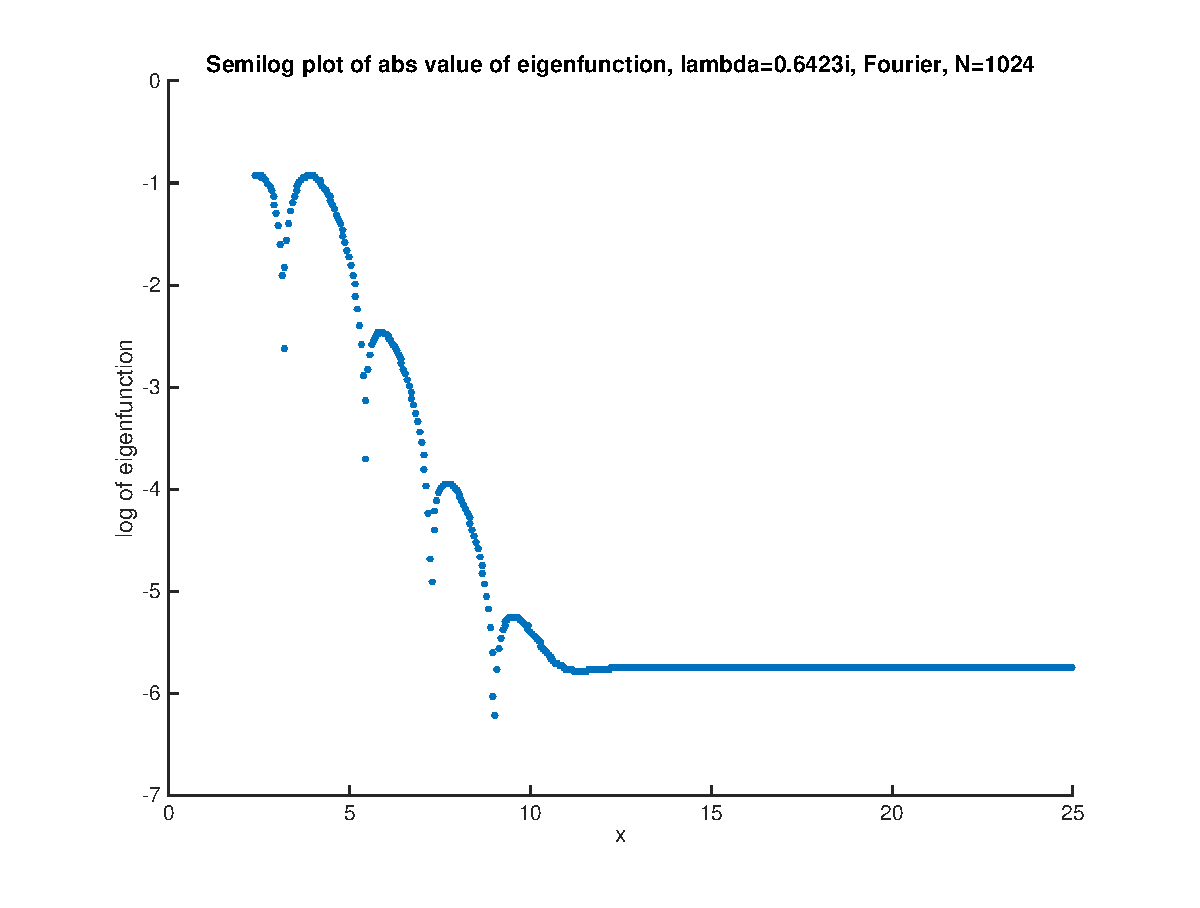
\includegraphics[width=8.5cm]{2doublesemilogeigenfn}
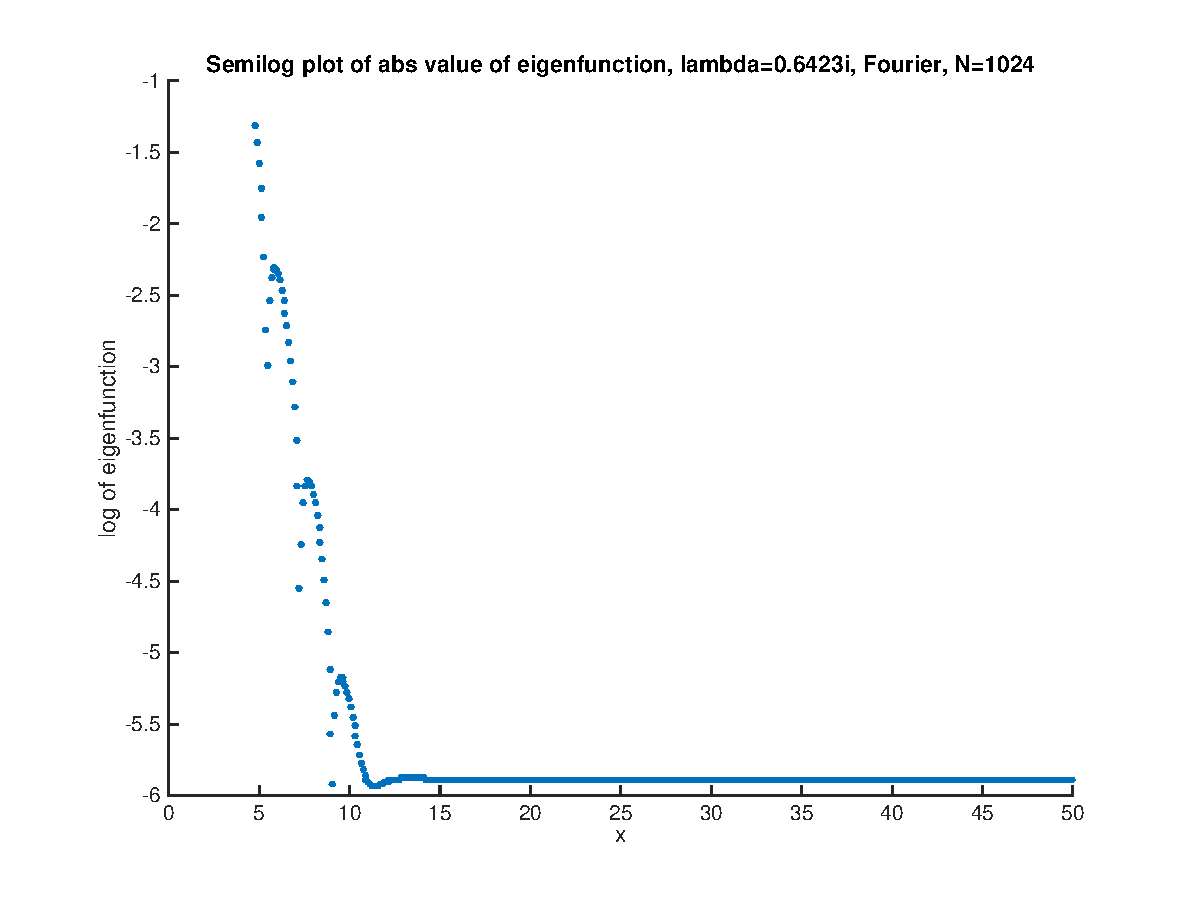
\includegraphics[width=8.5cm]{2doublesemilogeigenfn50}
\end{figure}

\subsubsection*{KdV, Double Pulse 4}
We can do the same thing for Double Pulse 4. Here we just show a semilog plot of the tail of the absolute value of the eigenfunction corresponding to $0.0215i$ for $L = 25$, Fourier spectral methods, and $N = 1024$. As in Double Pulse 2, we have exponential decay to a baseline, but the baseline is lower in this case, of approximate order $1e-8$.

\begin{figure}[H]
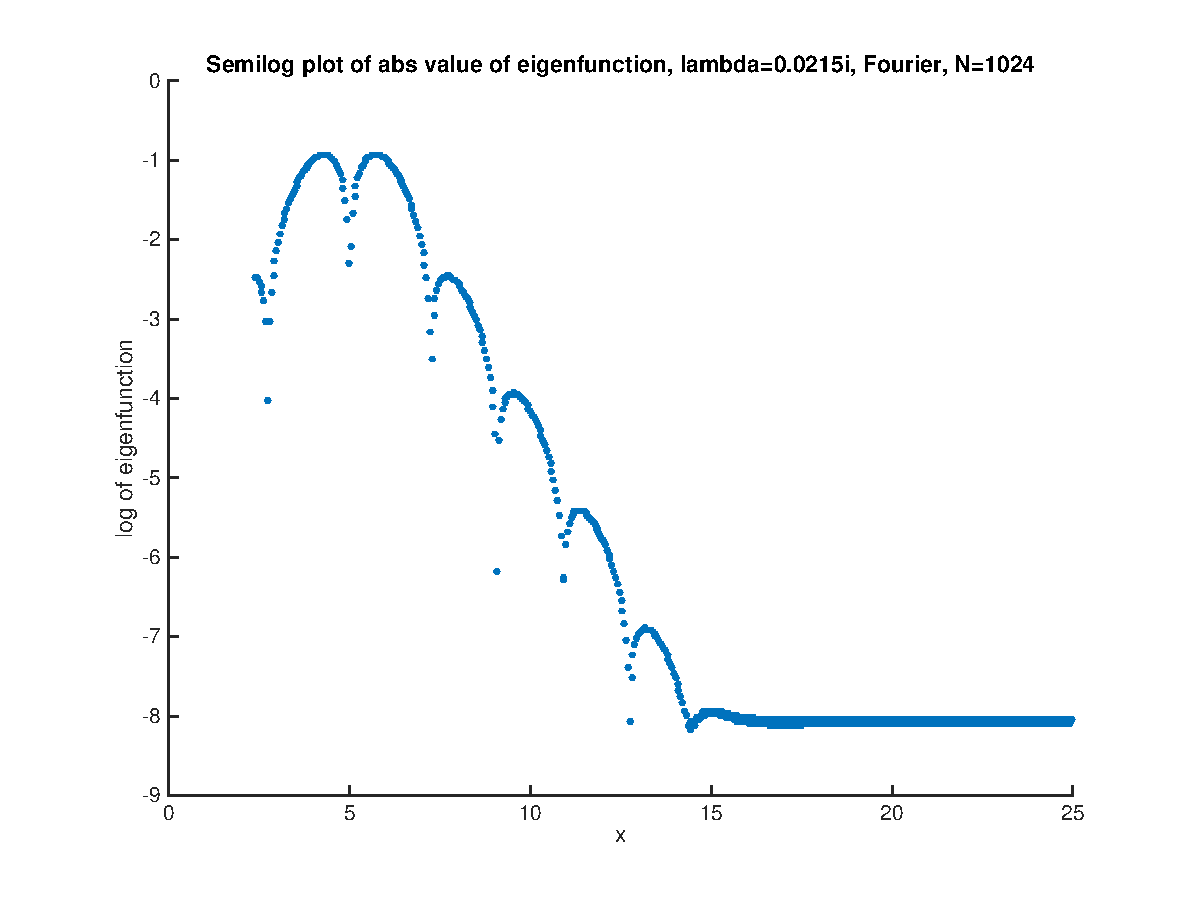
\includegraphics[width=8.5cm]{4doublesemilogeigenfn}
\end{figure}

\subsection*{Symmetry of Eigenfunctions}
The eigenfunctions corresponding to real eigenvalues are clearly not symmetric. We are thus interested in symmetry of eigenfunctions corresponding to the purely imaginary eigenvalues.

\subsubsection*{KdV, Double Pulse 2}
First, let's look at a plot of the absolute value of the eigenfunction.
\begin{figure}[H]
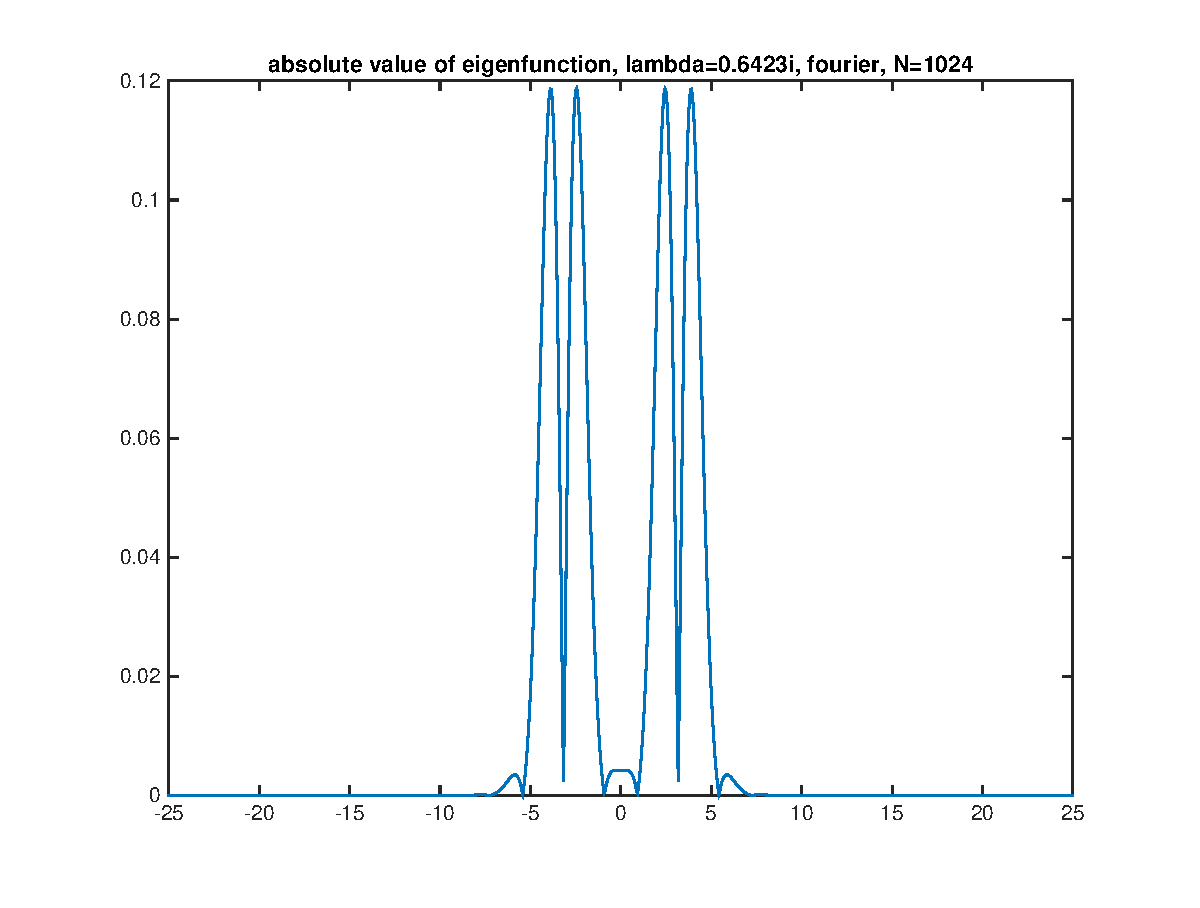
\includegraphics[width=8.5cm]{2doubleabseigenfn}
\end{figure}
Eyeballing this, it looks like it could be symmetric about $x = 0$. The peaks of the function are symmetric about $x = 0$, so that is a start. Calling the eigenfunction $v(x)$, let's check for symmetry of the absolute value by plotting $|v(x)| - |v(-x)|$.
\begin{figure}[H]
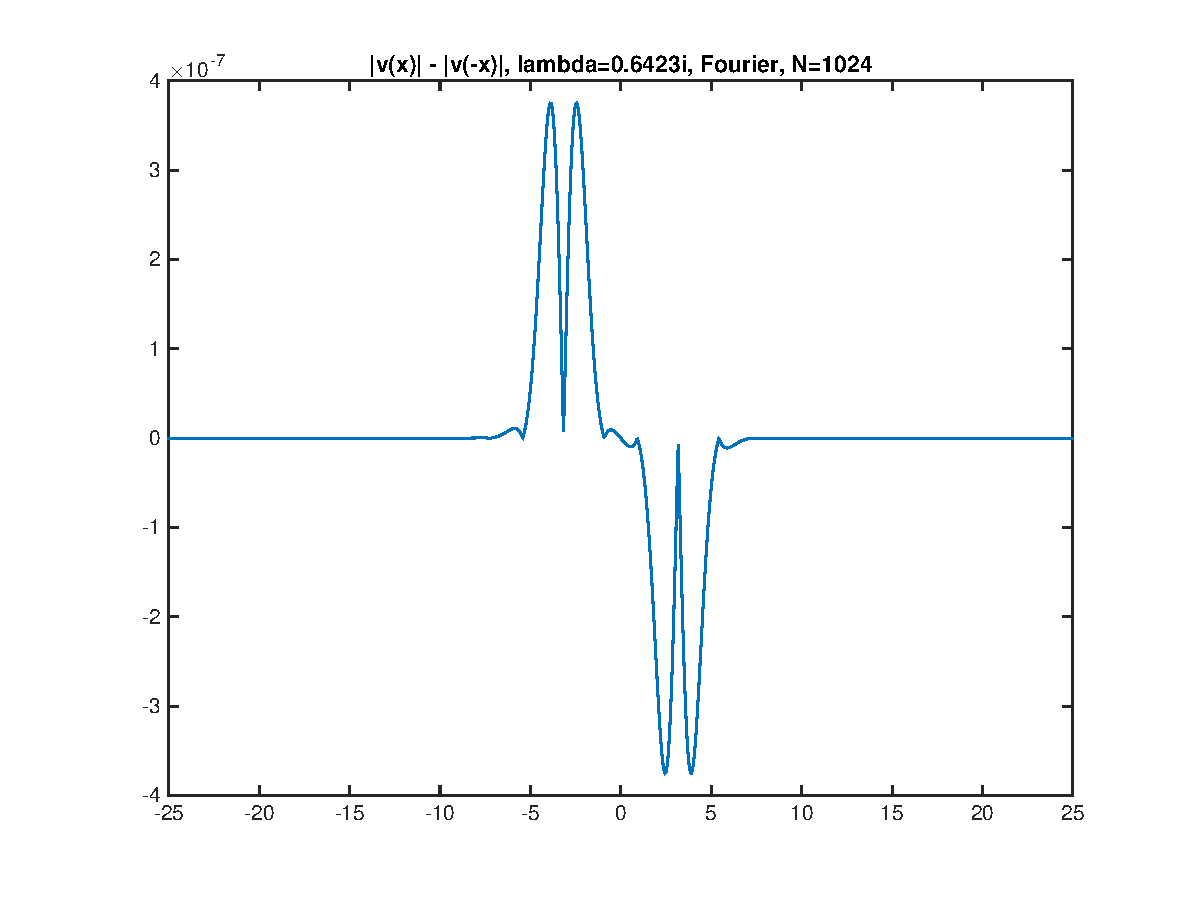
\includegraphics[width=8.5cm]{2doubleabseigenfnflipdiff}
\end{figure}
Although this is not zero, the max of the difference is of order $5e-7$, which is smaller than the baseline to which the eigenfunction decays. Increasing the number of grid points does not decrease this maximum, but increasing $L$ does. Here is a table of $\max{|v(x)| - |v(-x)|}$ for increasing $L$. We use $N = 2048$ for all of these to make sure we have enough grid points for the wave peaks.

\begin{figure}[H]
\begin{tabular}{l|ll}
  $N$   &  $L$   & $\max{|v(x)| - |v(-x)|}$ \\ \hline
        &        & $1.0e-05 *$            \\
  2048  &    25  &   0.1900 \\ 
  2048  &  37.5  &   0.0515 \\
  2048  &    50  &   0.0151 \\ 
  2048  &    75  &   0.0008 \\
  2048  &   100  &   0.0002 \\
  2048  &   125  &   0.0001 \\
\end{tabular}
\end{figure}

Plotting this on a log-log plot gives a reasonable straight line.

\begin{figure}[H]
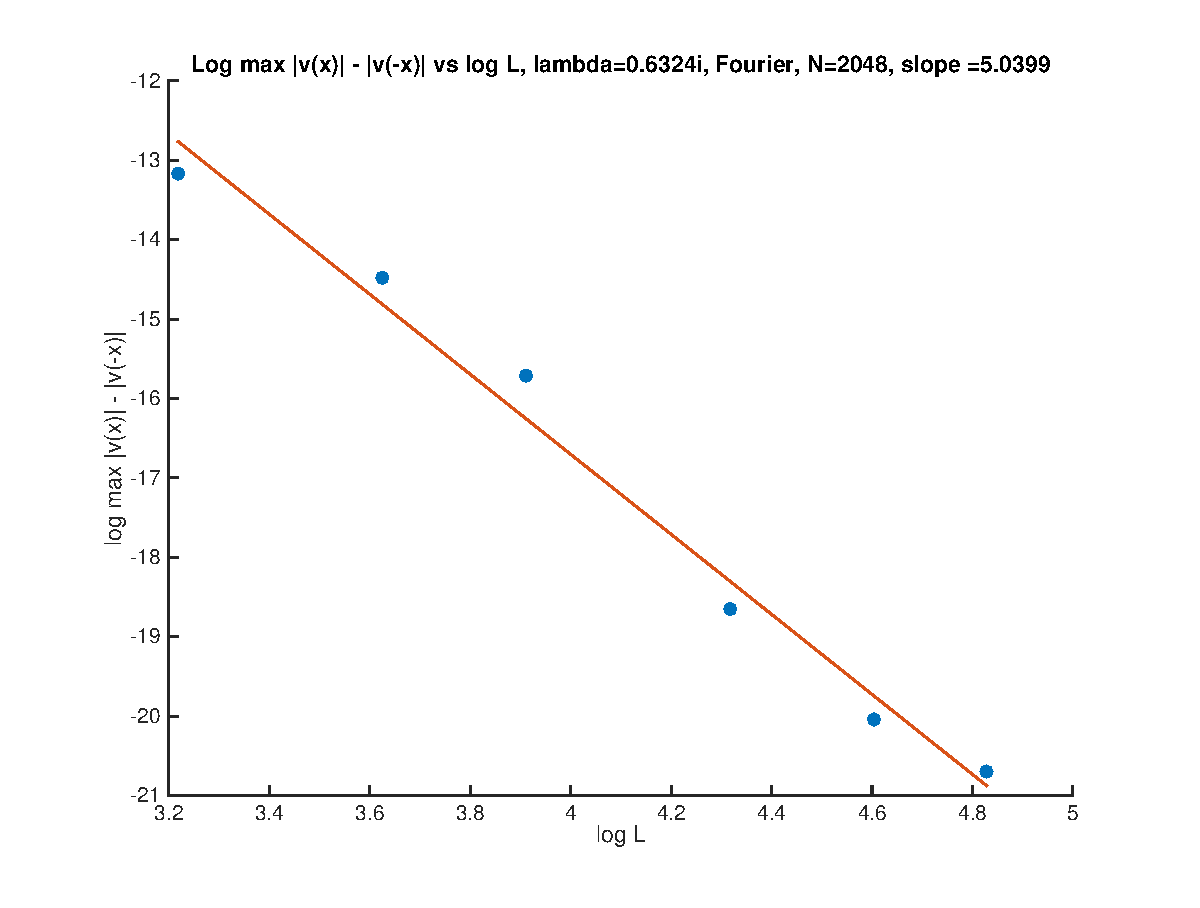
\includegraphics[width=8.5cm]{2doubleflipdiffloglogL}
\end{figure}
It is therefore reasonable to conclude that $|v(x)|$ is symmetric.

\subsubsection*{KdV, Double Pulse 4}
Here is a plot of the absolute value of the eigenfunction.
\begin{figure}[H]
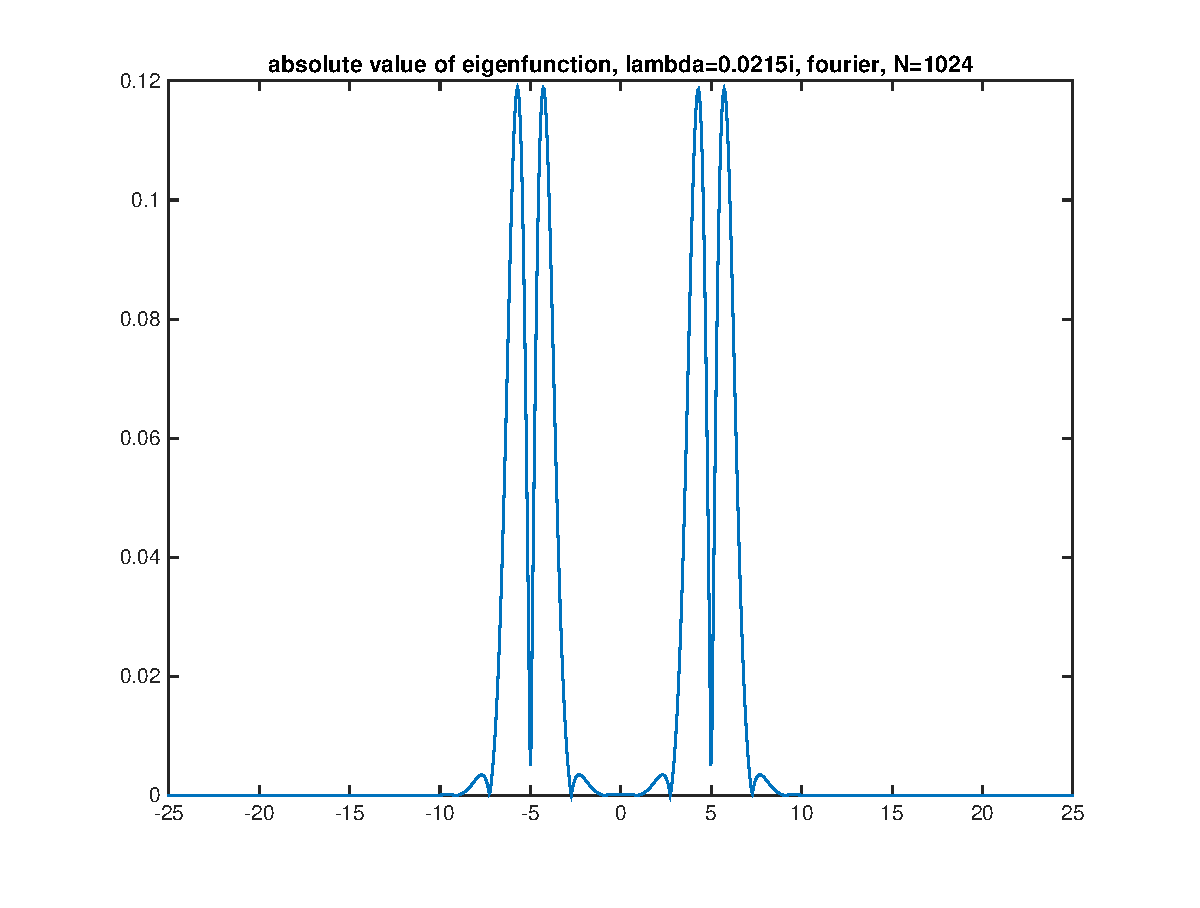
\includegraphics[width=8.5cm]{4doubleabseigenfn}
\end{figure}
Again, it looks like it could be symmetric about $x = 0$, but it's hard to tell. Let's check for symmetry of the absolute value by plotting $|v(x)| - |v(-x)|$ as before
\begin{figure}[H]
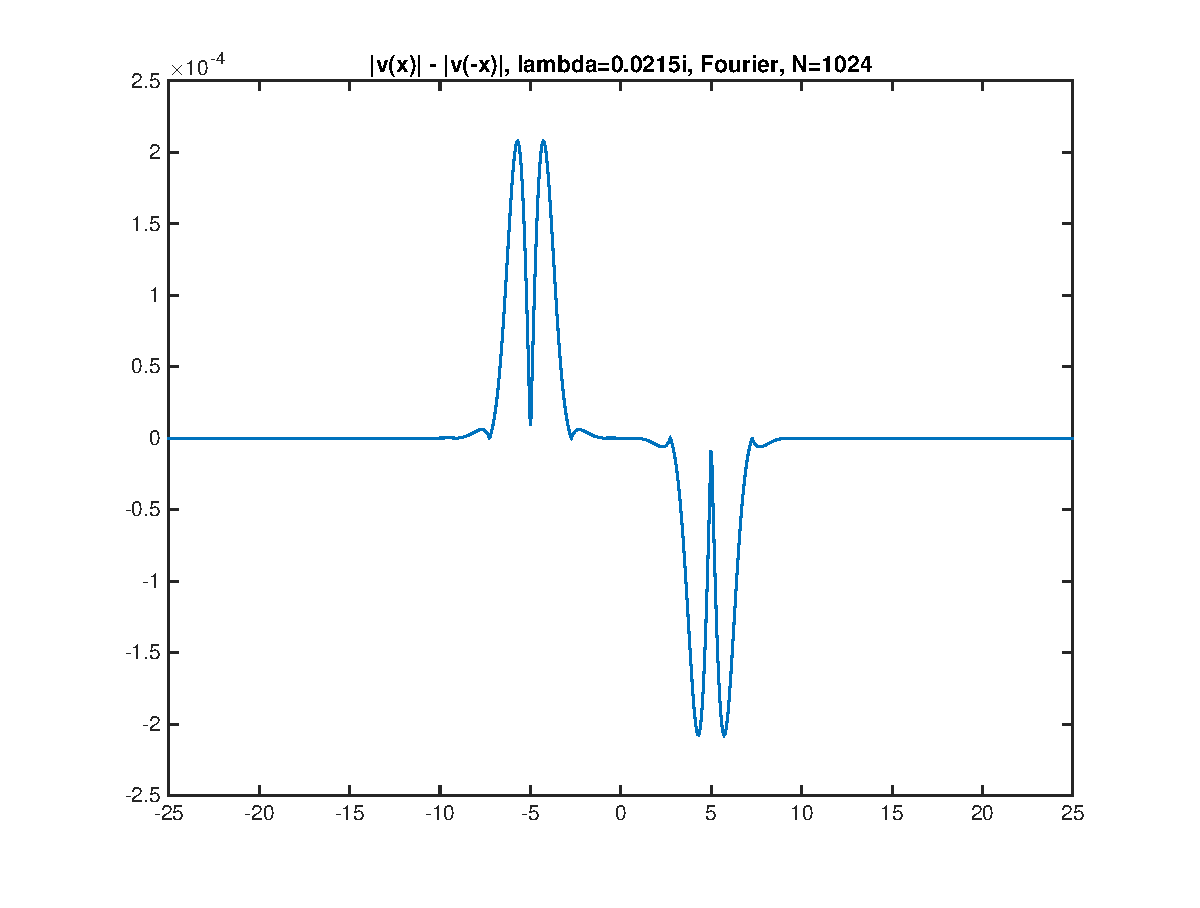
\includegraphics[width=8.5cm]{4doubleabseigenfnflipdiff}
\end{figure}
The max of the difference is of order $2e-4$, which is much larger than before. Increasing the number of grid points does not decrease this maximum. However, as with Double Pulse 2, increasing $L$ does decrease the max difference. Here is a table of $\max{|v(x)| - |v(-x)|}$ for increasing $L$. Again, we use $N = 2048$ for all of these to make sure we have enough grid points for the wave peaks.

\begin{figure}[H]
\begin{tabular}{l|ll}
  $N$   &  $L$   & $\max{|v(x)| - |v(-x)|}$ \\ \hline
  2048  &    25  &   0.0037 \\ 
  2048  &  37.5  &   5.8165e-04 \\
  2048  &    50  &   9.3905e-05 \\ 
  2048  &    60  &   3.7035e-05\\
  2048  &    75  &   1.5083e-05 \\
\end{tabular}
\end{figure}

Plotting this on a log-log plot again gives a reasonable straight line. The slope is similar to that for Double Pulse 4.

\begin{figure}[H]
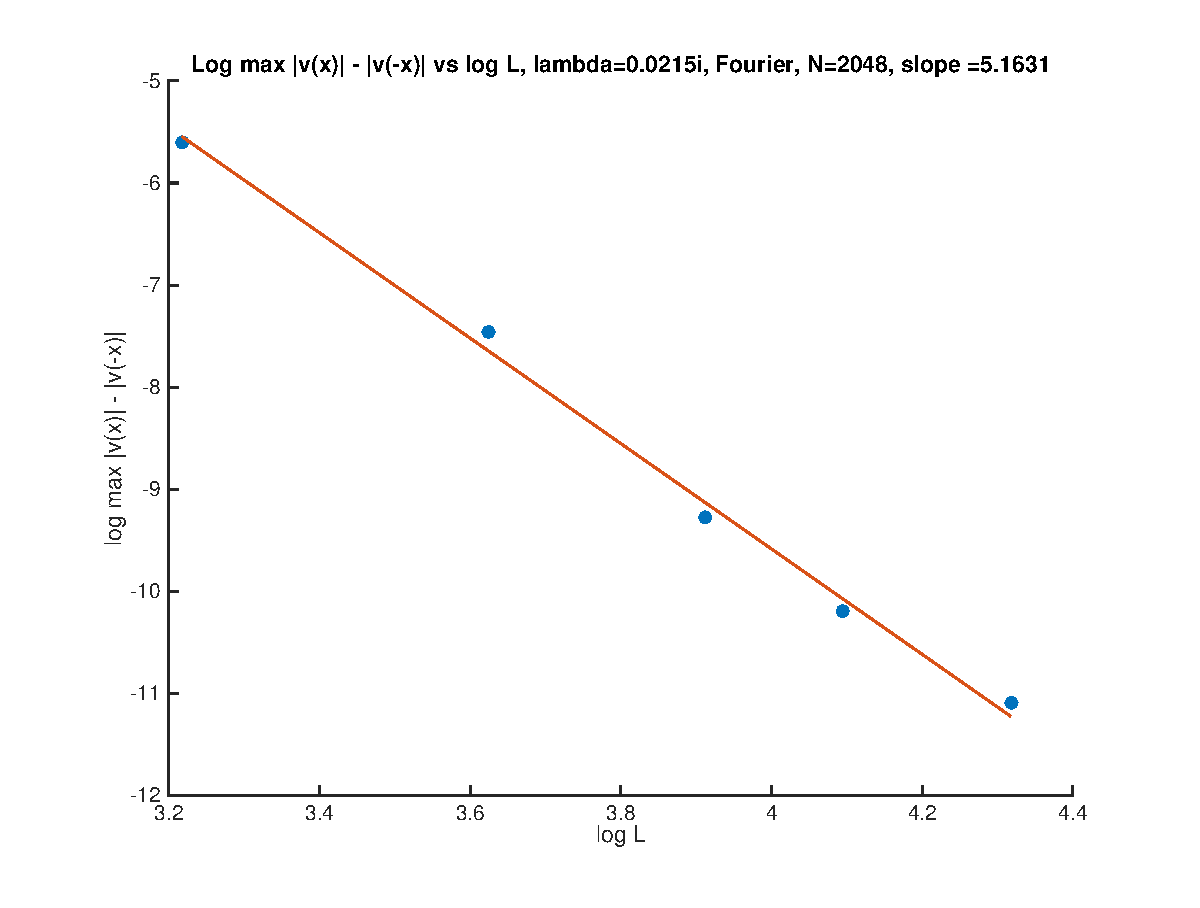
\includegraphics[width=8.5cm]{4doubleflipdiffloglogL}
\end{figure}
It is again reasonable to conclude that $|v(x)|$ is symmetric.

\end{document}
